\chapter{Основные части компонента управление УЗИ снимками}\label{app-format}
%\addcontentsline{toc}{chapter}{}

\begin{figure}[H]%
	\begin{center}
		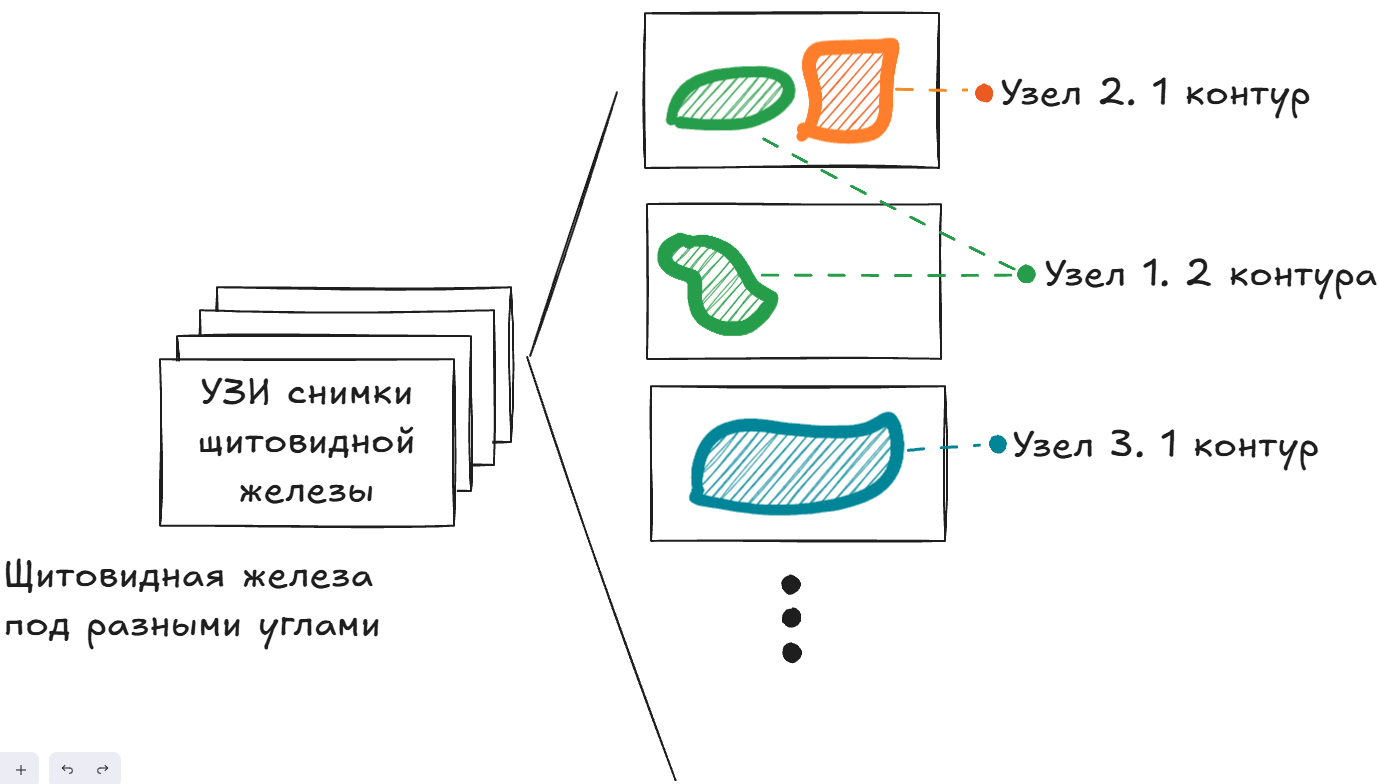
\includegraphics[width=.9\columnwidth]{./img/new/nodes_segments_model.png}%
	\end{center}
	\label{pic:seg_nod_model}%
\end{figure}

\begin{figure}[H]%
	\begin{center}
		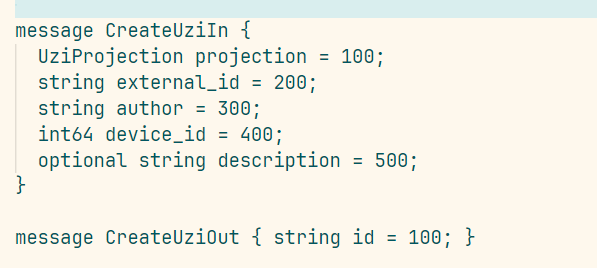
\includegraphics[width=.9\columnwidth]{./img/new/rpc_proto_2.png}%
	\end{center}
	\label{pic:rpc_2_message}%
\end{figure}


\lstinputlisting[
  label=lst:uzi_service.proto,
  float=tb,frame=lines,
  caption=Контракт компонента управление УЗИ снимками
]{listings/uzi_service.proto}

\lstinputlisting[
  label=lst:uziupload.proto,
  float=tb,frame=lines,
  caption=Листинг топика \texttt{uziupload}
]{listings/uziupload.proto}

\lstinputlisting[
  label=lst:uzisplitted.proto,
  float=tb,frame=lines,
  caption=Листинг топика \texttt{uzisplitted}
]{listings/uzisplitted.proto}

\lstinputlisting[
  label=lst:uziprocessed.proto,
  float=tb,frame=lines,
  caption=Листинг топика \texttt{uziprocessed}
]{listings/uziprocessed.proto}

\lstinputlisting[
  label=lst:node_controller_hadnler.go,
  float=tb,frame=lines,
  caption=Контроллер gRPC ручек для взаимодействия с узлами
]{listings/node_controller_hadnler.go}

\lstinputlisting[
  label=lst:node_get_handler.go,
  float=tb,frame=lines,
  caption=Контроллер gRPC ручки получения узла узи
]{listings/node_get_handler.go}

\lstinputlisting[
  label=lst:create_nodes_1.go,
  float=tb,frame=lines,
  caption=Создание нового узла с сегментами ч.1
]{listings/create_nodes_1.go}

\lstinputlisting[
  label=lst:create_nodes_2.go,
  float=tb,frame=lines,
  caption=Создание нового узла с сегментами ч.2
]{listings/create_nodes_2.go}

\lstinputlisting[
  label=lst:uzi_1.sql,
  float=tb,frame=lines,
  caption=Создание бд узи компонента ч.1
]{listings/uzi_1.sql}

\lstinputlisting[
  label=lst:uzi2.sql,
  float=tb,frame=lines,
  caption=Создание бд узи компонента ч.2
]{listings/uzi2.sql}




% Текст пояснительной записки должен готовиться для печати на листах формата А4, использоваться должен шрифт с засечками (Roman; обычно --- Times Roman или Times New Roman), 12 или 14 кегль. Размеры полей:

% \begin{itemize}
% 	\item верхнее: 20 мм.
% 	\item нижнее: 20 мм.
% 	\item левое: 10 мм.
% 	\item правое: 25 мм.
% \end{itemize}

% Нумероваться должны все страницы, начиная с первой (титульной), однако сами номера следует проставлять на страницах, начиная со страницы реферата. Номер следует проставлять внизу страницу (в центре).

% Заголовки оформляются тем же шрифтом, что и основной текст (т.е., соответственно, Times Roman или Times New Roman). Для заголовков первого уровня размер шрифта может быть больше размера шрифта основного текста (обычно 14-16).

% Все разделы текста: реферат, оглавление, введение, три главы основного
% содержания, список литературы, заключение, приложения --- должны снабжаться
% содержательным заголовком и начинаться с новой страницы; сами заголовки следует
% при этом центрировать (заголовки параграфов и пунктов выравниваются по ширине).
% Следует обратить внимание, что заголовки всех разделов, кроме трех основных
% глав, регламентированы; заголовки трех основных глав должны быть содержательными
% и отражать суть соответствующей главы. Названия типа <<Аналитическая часть>> и <<Теоретическая глава>> --- \textit{недопустимы}.

% Текст пояснительной записки может содержать рисунки и таблицы. Все рисунки и
% таблицы должны снабжаться номерами и подписями:

% \begin{itemize}

% 	\item нумерация рисунков и таблиц должна быть сквозная (но раздельная, т.к. для рисунков своя, для таблиц --- своя);

% 	\item в случае большого количества иллюстраций/таблиц, допускается <<вложенная>> нумерация (т.е. таблицу/рисунок можно снабжать составным номером в формате 
	
% 	$$\langle\mbox{номер главы}\rangle.\langle\mbox{номер внутри главы}\rangle;$$
	
% 	\item подрисуночная подпись должна располагаться снизу по центру;
	
% 	\item название таблицы следует помещать над таблицей слева, без абзацного
% 	отступа в одну строку с ее номером через тире (ГОСТ 7.32-2001, п.6.6.1).

% \end{itemize}

% Здесь перечислены не все, а лишь основные требования к оформлению. Прочие
% требования --- см. соответствующие ГОСТы.

% Для того чтобы избежать больших отступов в списках, которые по умолчанию добавляют окружения \texttt{itemize} и \texttt{enumerate}, следует использовать 
% \texttt{compactitem} (для маркированных списков) и \texttt{compactenum} (для нумерованных списков) из пакета \texttt{paralist}. 
% Например:

% \begin{compactitem}
% 	\item это;
% 	\item не нумерованный;
% 	\item список;
% 	\item без лишних промежутков.
% \end{compactitem}

% И для нумерованных списков:

% \begin{compactenum}[1)]
% 	\item нумерованные списки;
% 	\item пакета \texttt{paralist};
% 	\item еще и удобно настраивать;
% 	\item (например, менять формат номера).
% \end{compactenum}

% \noindent или

% \begin{compactenum}[a)]
% 	\item это другой;
% 	\item нумерованный;
% 	\item список;
% 	\item без лишних промежутков;
% 	\item и с буквенной нумерацией.
% \end{compactenum}

% А если хочется нумерацию сделать ангоязычной, то нужно использовать окружение \texttt{other\-language} (таким образом: \verb|\begin{otherlanguage}[numerals=latin]{russian}|)

% \setkeys{russian}{numerals=latin}
% %\selectlanguage{russian}
% %\begin{otherlanguage}[numerals=latin]{russian}
% \begin{russian}
% \begin{compactenum}[a)]
% 	\item это другой;
% 	\item нумерованный;
% 	\item список;
% 	\item без лишних промежутков;
% 	\item и с буквенной нумерацией.
% \end{compactenum}
% \end{russian}
% %\end{otherlanguage}

% \textbf{Замечание.} По неизвестным причинам, переключения не происходит, хотя должно.

%%% Local Variables:
%%% TeX-engine: xetex
%%% eval: (setq-local TeX-master (concat "../" (seq-find (-cut string-match ".*-3-pz\.tex$" <>) (directory-files ".."))))
%%% End:
